\documentclass[defaultstyle,11pt]{thesis}

\usepackage{amsmath}
\usepackage{amssymb}		% to get all AMS symbols
\usepackage{graphicx}		% to insert figures
\usepackage{mystyle}

%%%%%%%%%%%%   All the preamble material:   %%%%%%%%%%%%

\title{This is the Name of my Thesis}

\author{I.~B.}{Scriptor}

\otherdegrees{B.A., North Dakota State University, 2005 \\
	      M.S., University of Reno, 2007}

\degree{Doctor of Philosophy}		%  #1 {long descr.}
	{Ph.D., Physics}		%  #2 {short descr.}

\dept{Department of}			%  #1 {designation}
	{Physics}		%  #2 {name}

\advisor{Prof.}				%  #1 {title}
	{Anna Hasenfratz}			%  #2 {name}

\reader{Prof.~Rachel Goddard}		%  2nd person to sign thesis
\readerThree{Ms.~Thora Nea}		%  3rd person to sign thesis

\abstract{  \OnePageChapter	% because it is very short

	Often the abstract will be long enough to require
	more than one page, in which case the macro
	``$\backslash$OnePageChapter'' should {\it not}
	be used.

	But this one isn't, so it should.
	}

\dedication[Dedication]{	% NEVER use \OnePageChapter here.
	To all of the fluffy kitties.
	}

\acknowledgements{	\OnePageChapter	% *MUST* BE ONLY ONE PAGE!
	Here's where you acknowledge folks who helped.
	But keep it short, i.e., no more than one page,
	as required by the Grad School Specifications.
	}

% \IRBprotocol{E927F29.001X}	% optional!

\ToCisShort	% use this only for 1-page Table of Contents

\LoFisShort	% use this only for 1-page Table of Figures
% \emptyLoF	% use this if there is no List of Figures

\LoTisShort	% use this only for 1-page Table of Tables
% \emptyLoT	% use this if there is no List of Tables

%%%%%%%%%%%%%%%%%%%%%%%%%%%%%%%%%%%%%%%%%%%%%%%%%%%%%%%%%%%%%%%%%
%%%%%%%%%%%%%%%       BEGIN DOCUMENT...         %%%%%%%%%%%%%%%%%
%%%%%%%%%%%%%%%%%%%%%%%%%%%%%%%%%%%%%%%%%%%%%%%%%%%%%%%%%%%%%%%%%

\begin{document}

  \chapter{Introduction}
\label{ch:introduction}

  \section{Abstract}
  \label{sec:abstract}
  % 1.1
% Motivation

Strongly coupled quantum field theories play a vial part in our current understanding of the universe.



  \section{Organization}
  \label{sec:organization}
  % 2.2
% Higgs Mechanism

In the standard model the $W^{\pm}$ and $Z$ bosons are massive but the photon is massless.
Since gauge invariance dictates that a mass term is forbidden in the Lagrangian, this seems to pose a problem.
Disaster is averted because $SU(2)_W \times U(1)_Y$ is spontaneously broken to $U(1)_{EM}$.
In the standard model this is accomplished by adding a complex scalar doublet field to the theory.
The field is named the Higgs field after one of its discoverers.
The following discussion shows how electroweak symmetry breaking is facilitated by the Higgs \cite{Quigg:ds52, Quigg:ds53, peskin:book}.

Lets introduce a complex elementary scalar doublet $\Phi=\left(\begin{matrix}\phi^+\\\phi_0\end{matrix}\right)$ that transforms in the (1,2,$\frac{1}{2}$) representation of $SU(3)_C\times SU(2)_L\times U(1)_Y$.
We allow all terms in the Lagrangian that have mass dimension $\leq 4$, thus ignoring irrelevant operators,
\begin{equation}
  \Lagr_H=(D_\mu\Phi)^\dagger(D^\mu\Phi)+\mu^2\Phi^\dagger\Phi-|\lambda|(\Phi^\dagger\Phi)^2,
\end{equation}
with covariant derivative
\begin{equation}
  D_\mu\Phi=(\partial_\mu-igA^a_\mu\tau^a-ig'YB_\mu)\Phi.
\end{equation}
$A^a_\mu$ and $B_\mu$ are the $SU(2)$ and $U(1)$ gauge bosons respectively.
The coupling constant $g$ belongs to $SU(2)$ and the coupling constant $g'$ belongs to $U(1)$.
Finally $Y$ is the generator of hypercharge, $\tau^a$ are the generators of $SU(2)$ and are related to the Pauli matrices
\begin{equation}
  \tau^a=\frac{1}{2}\sigma^a.
\end{equation}

We can now identify the potential $V(\Phi)$ as
\begin{equation}
  V(\Phi)=-\mu^2\Phi^\dagger\Phi+|\lambda|(\Phi^\dagger\Phi)^2,
\end{equation}
this potential is shown in figure \ref{fig:higgspot}.
As long as $\mu^2$ is positive the potential has a spontaneously broken symmetry.
Gauge invariance allows us to choose the vacuum state to correspond to the vacuum expectation value (VEV)
\begin{equation}
  \left<\Phi\right>_0=\frac{\nu}{\sqrt{2}}\left(\begin{matrix}0 \\ \nu\end{matrix}\right),
\end{equation}
where $\nu=\sqrt{\frac{\mu^2}{|\lambda|}}$.
Moreover, $\nu$ is related to the Fermi constant, $G_F$, by
\begin{equation}
  \nu=\frac{1}{2^{1/4}\sqrt{G_F}}\approx 246 \mbox{ GeV}.
\end{equation}

\begin{figure}[h]
  \begin{center}
    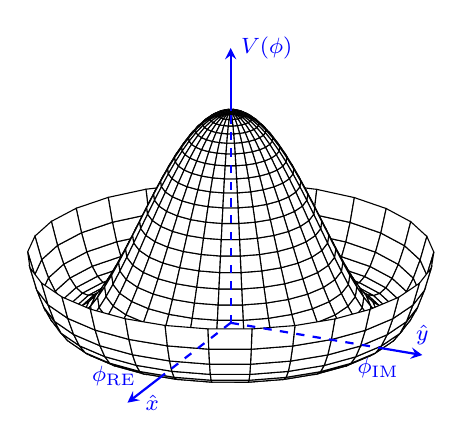
\begin{tikzpicture}
        \begin{axis}[
            hide axis,
            %axis lines=middle,
%            axis on top,
%            axis line style={blue,dashed,thick},
%            ymin=-2,ymax=2,
%            xmin=-2,xmax=2,
%            zmin=-2,zmax=2,
            samples=30,
            domain=0:360,
            y domain=0:1.25,clip=false
        ]
        \addplot3 [surf, shader=flat, draw=black, fill=white, z buffer=sort]
           ({sin(x)*y}, {cos(x)*y}, {(y^2-1)^2});
        \draw[blue,thick,dashed] (axis cs:0,0,0) -- (axis cs:1,0,0)
                    node[below,font=\footnotesize]{$\phi_{\text{IM}}$};
        \draw[blue,thick,-stealth] (axis cs:1,0,0) -- (axis cs:1.3,0,0)
                    node[above,font=\footnotesize]{$\hat{y}$};
        \draw[blue,thick,dashed] (axis cs:0,0,0) -- (axis cs:0,-1,0)
                    node[left=2mm,font=\footnotesize]{$\phi_{\text{RE}}$};
        \draw[blue,thick,-stealth] (axis cs:0,-1,0) -- (axis cs:0,-1.5,0)
                    node[right=1mm,font=\footnotesize]{$\hat{x}$};
        \draw[blue,thick,dashed] (axis cs:0,0,0) -- (axis cs:0,0,1)
                    %node[left=2mm,font=\footnotesize]{$\phi_{\text{RE}}$}
                    ;
        \draw[blue,thick,-stealth] (axis cs:0,0,1) -- (axis cs:0,0,1.3)
        node[right,font=\footnotesize]{$V(\phi)$};
        \end{axis}
    \end{tikzpicture}
  \end{center}
  \caption{The Higgs potential with $\mu^2>0$ has a spontaneously broken global symmetry.  We can think of this classically. The origin is a local maximum of potential energy and therefore an unstable equilibrium. If we place a particle at the origin any perturbation will push the particle `down hill' to a minimum of the potential.  Since there are a number of degenerate minima, choosing one spontaneously breaks the symmetry.}
  \label{fig:higgspot}
\end{figure}


If we assign our theory to have hypercharge $Y=+\frac{1}{2}$, a complete gauge transformation in this theory is
\begin{equation}
  \Phi\rightarrow e^{i\alpha^a(x)\tau^a}e^{i\beta(x)/2}\Phi.
\end{equation}
Making the particluar choice of $\alpha^1=\alpha^2=0$ and $\alpha^3=\beta$ we see that $\left<\Phi\right>$ is invariant.
Therefore the theory still contains an unbroken U(1) symmetry which we identify with electromagnetism.
This unbroken U(1) symmetry contains one massless gauge boson which is the photon.
The other three gauge bosons corresponding to the broken generators of the symmetry group become massive.
The massive gauge bosons get their mass from the square of the kinetic term evaluated at the VEV
\begin{equation}
  (D_\mu\Phi)^\dagger(D^\mu\Phi)=\frac{1}{2}(\begin{matrix}0& \nu\end{matrix})\Big(gA^a_\mu\tau^a+\frac{1}{2}g'B_\mu\Big)\Big(gA^{b\mu}\tau^\mu+\frac{1}{2}g'B^\mu\Big)\left(\begin{matrix}0\\\nu\end{matrix}\right).
\end{equation}
Substituting $\tau^a$ and taking the product we get
\begin{equation}
  (D_\mu\Phi)^\dagger(D^\mu\Phi)=\frac{\nu^2}{8}\Big[g^2(A^1_\mu)^2+g^2(A^2_\mu)^2+(-gA^3_\mu+g'B_\mu)^2\Big].
\end{equation}
We can now perform a field redefinition and recover
\begin{align}
  W^\pm_\mu&=\frac{1}{\sqrt{2}}\Big(A^1_\mu\mp A^2_\mu\Big)&\mbox{\quad with mass\quad} m_W=g\frac{\nu}{2}\\
  Z_\mu&=\frac{1}{\sqrt{g^2+g'^2}}\Big(gA^3_\mu-g'B_\mu\Big)&\mbox{\quad with mass\quad} m_Z=\sqrt{g^2+g'^2}\frac{\nu}{2}\\
  A_\mu&=\frac{1}{\sqrt{g^2+g'^2}}\Big(g'A^3_\mu+gB_\mu\Big)&\mbox{\quad with mass\quad} m_A=0,
\end{align}
which are the standard model $W^\pm, Z$ bosons and photon.

The change in basis from the original massless bosons to massive bosons and photon is characterized by the weak mixing angle $\theta_w$:
\begin{equation}
  \left(\begin{matrix}Z_\mu\\A_\mu\end{matrix}\right)=\left(\begin{matrix}\cos\theta_w & -\sin\theta_w\\\sin\theta_w & \cos\theta_w\end{matrix}\right)\left(\begin{matrix}A^3_\mu\\ B_\mu\end{matrix}\right),
\end{equation}
with
\begin{equation}
  \cos\theta_w=\frac{g}{\sqrt{g^2+g'^2}},\quad\sin\theta_w=\frac{g'}{\sqrt{g^2+g'^2}}.
\end{equation}

When the $W^\pm$ and $Z$ bosons become massive they each gain an additional longitudinal degree of freedom.
These new degrees of freedom aren't free; they come from the three components of the Higgs doublet $\Phi$ associated with the original broken symmetry.
The Goldstone mechanism facilitates this transfer of degrees of freedom.
The vernacular is that the massless Goldstone bosons of the original theory are ``eaten" by the $W^\pm$ and $Z$.


Additionally, the Higgs mechanism provides a mass for the standard model fermions.
Fermion mass terms are forbidden in the standard model because they would violate local gauge invariance since left and right fermions transform differently.
Now that we have a scalar field $\Phi$ we can couple it to our fermion with a Yukawa coupling, $-c\bar{f_L}\Phi f_R$.
In such a term $f_L$ and $f_R$ are the right and left components of the fermion, $c$ is an arbitrary coupling characterizing the strength of the interaction with the Higgs VEV, and $\Phi$ is the Higgs VEV.
Heavy particles like the top have a large value of $c$ while light particles like the up quark have a small value of $c$.

Finally, the Higgs Boson, a particle excitations of the Higgs field, was recently discovered at the Large Hadron Collider (LHC).The discovery was announced to the pulbic July 4, 2012.
Current experimental results pin the Higgs mass at 126 GeV.
Peter Higgs and François Englert shared the Nobel prize in 2013 for their work in developing the theory of EWSB through the Higgs mechanism.


  \chapter{Strongly Coupled Physics Beyond the Standard Model}
\label{ch:strongdynamics}

\section{The Standard Model}
\label{sec:sm}
\input{\cnum{2}/section_1}

\section{Higgs Mechanism}
\label{sec:higgs_mech}
\input{\cnum{2}/section_2}

\section{Beyond Standard Model Physics}
\label{sec:beyond_sm}
\input{\cnum{2}/section_3}

\section{Composite Higgs}
\label{sec:composite_higgs}
\input{\cnum{2}/section_4}

  \chapter{Lattice Field Theory}
\label{ch:lattice}

  \chapter{Monte Carlo Renormalization Group}
\label{ch:MCRG}


  \section{Introduction}
  \label{sec:MCRG-intro}
  \input{\cnum{4}/section_1}

  \section{Method}
  \label{sec:MCRG-method}
  \input{\cnum{4}/section_2}

  \section{8 and 12 Flavor Results}
  \label{sec:MCRG-matching}
  \input{\cnum{4}/section_3}

  \section{Summary}
  \label{sec:MCRG-summary}
  \input{\cnum{4}/section_4}

  \chapter{Running Coupling and the Renormalization Group}
\label{ch:theory}

  \section{Running Coupling}
  \label{sec:rc}
  % 1.1
% Motivation

Strongly coupled quantum field theories play a vial part in our current understanding of the universe.



  \section{Renormalization Group}
  \label{sec:rg}
  % 2.2
% Higgs Mechanism

In the standard model the $W^{\pm}$ and $Z$ bosons are massive but the photon is massless.
Since gauge invariance dictates that a mass term is forbidden in the Lagrangian, this seems to pose a problem.
Disaster is averted because $SU(2)_W \times U(1)_Y$ is spontaneously broken to $U(1)_{EM}$.
In the standard model this is accomplished by adding a complex scalar doublet field to the theory.
The field is named the Higgs field after one of its discoverers.
The following discussion shows how electroweak symmetry breaking is facilitated by the Higgs \cite{Quigg:ds52, Quigg:ds53, peskin:book}.

Lets introduce a complex elementary scalar doublet $\Phi=\left(\begin{matrix}\phi^+\\\phi_0\end{matrix}\right)$ that transforms in the (1,2,$\frac{1}{2}$) representation of $SU(3)_C\times SU(2)_L\times U(1)_Y$.
We allow all terms in the Lagrangian that have mass dimension $\leq 4$, thus ignoring irrelevant operators,
\begin{equation}
  \Lagr_H=(D_\mu\Phi)^\dagger(D^\mu\Phi)+\mu^2\Phi^\dagger\Phi-|\lambda|(\Phi^\dagger\Phi)^2,
\end{equation}
with covariant derivative
\begin{equation}
  D_\mu\Phi=(\partial_\mu-igA^a_\mu\tau^a-ig'YB_\mu)\Phi.
\end{equation}
$A^a_\mu$ and $B_\mu$ are the $SU(2)$ and $U(1)$ gauge bosons respectively.
The coupling constant $g$ belongs to $SU(2)$ and the coupling constant $g'$ belongs to $U(1)$.
Finally $Y$ is the generator of hypercharge, $\tau^a$ are the generators of $SU(2)$ and are related to the Pauli matrices
\begin{equation}
  \tau^a=\frac{1}{2}\sigma^a.
\end{equation}

We can now identify the potential $V(\Phi)$ as
\begin{equation}
  V(\Phi)=-\mu^2\Phi^\dagger\Phi+|\lambda|(\Phi^\dagger\Phi)^2,
\end{equation}
this potential is shown in figure \ref{fig:higgspot}.
As long as $\mu^2$ is positive the potential has a spontaneously broken symmetry.
Gauge invariance allows us to choose the vacuum state to correspond to the vacuum expectation value (VEV)
\begin{equation}
  \left<\Phi\right>_0=\frac{\nu}{\sqrt{2}}\left(\begin{matrix}0 \\ \nu\end{matrix}\right),
\end{equation}
where $\nu=\sqrt{\frac{\mu^2}{|\lambda|}}$.
Moreover, $\nu$ is related to the Fermi constant, $G_F$, by
\begin{equation}
  \nu=\frac{1}{2^{1/4}\sqrt{G_F}}\approx 246 \mbox{ GeV}.
\end{equation}

\begin{figure}[h]
  \begin{center}
    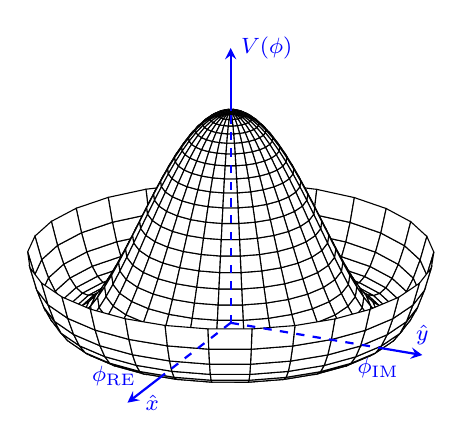
\begin{tikzpicture}
        \begin{axis}[
            hide axis,
            %axis lines=middle,
%            axis on top,
%            axis line style={blue,dashed,thick},
%            ymin=-2,ymax=2,
%            xmin=-2,xmax=2,
%            zmin=-2,zmax=2,
            samples=30,
            domain=0:360,
            y domain=0:1.25,clip=false
        ]
        \addplot3 [surf, shader=flat, draw=black, fill=white, z buffer=sort]
           ({sin(x)*y}, {cos(x)*y}, {(y^2-1)^2});
        \draw[blue,thick,dashed] (axis cs:0,0,0) -- (axis cs:1,0,0)
                    node[below,font=\footnotesize]{$\phi_{\text{IM}}$};
        \draw[blue,thick,-stealth] (axis cs:1,0,0) -- (axis cs:1.3,0,0)
                    node[above,font=\footnotesize]{$\hat{y}$};
        \draw[blue,thick,dashed] (axis cs:0,0,0) -- (axis cs:0,-1,0)
                    node[left=2mm,font=\footnotesize]{$\phi_{\text{RE}}$};
        \draw[blue,thick,-stealth] (axis cs:0,-1,0) -- (axis cs:0,-1.5,0)
                    node[right=1mm,font=\footnotesize]{$\hat{x}$};
        \draw[blue,thick,dashed] (axis cs:0,0,0) -- (axis cs:0,0,1)
                    %node[left=2mm,font=\footnotesize]{$\phi_{\text{RE}}$}
                    ;
        \draw[blue,thick,-stealth] (axis cs:0,0,1) -- (axis cs:0,0,1.3)
        node[right,font=\footnotesize]{$V(\phi)$};
        \end{axis}
    \end{tikzpicture}
  \end{center}
  \caption{The Higgs potential with $\mu^2>0$ has a spontaneously broken global symmetry.  We can think of this classically. The origin is a local maximum of potential energy and therefore an unstable equilibrium. If we place a particle at the origin any perturbation will push the particle `down hill' to a minimum of the potential.  Since there are a number of degenerate minima, choosing one spontaneously breaks the symmetry.}
  \label{fig:higgspot}
\end{figure}


If we assign our theory to have hypercharge $Y=+\frac{1}{2}$, a complete gauge transformation in this theory is
\begin{equation}
  \Phi\rightarrow e^{i\alpha^a(x)\tau^a}e^{i\beta(x)/2}\Phi.
\end{equation}
Making the particluar choice of $\alpha^1=\alpha^2=0$ and $\alpha^3=\beta$ we see that $\left<\Phi\right>$ is invariant.
Therefore the theory still contains an unbroken U(1) symmetry which we identify with electromagnetism.
This unbroken U(1) symmetry contains one massless gauge boson which is the photon.
The other three gauge bosons corresponding to the broken generators of the symmetry group become massive.
The massive gauge bosons get their mass from the square of the kinetic term evaluated at the VEV
\begin{equation}
  (D_\mu\Phi)^\dagger(D^\mu\Phi)=\frac{1}{2}(\begin{matrix}0& \nu\end{matrix})\Big(gA^a_\mu\tau^a+\frac{1}{2}g'B_\mu\Big)\Big(gA^{b\mu}\tau^\mu+\frac{1}{2}g'B^\mu\Big)\left(\begin{matrix}0\\\nu\end{matrix}\right).
\end{equation}
Substituting $\tau^a$ and taking the product we get
\begin{equation}
  (D_\mu\Phi)^\dagger(D^\mu\Phi)=\frac{\nu^2}{8}\Big[g^2(A^1_\mu)^2+g^2(A^2_\mu)^2+(-gA^3_\mu+g'B_\mu)^2\Big].
\end{equation}
We can now perform a field redefinition and recover
\begin{align}
  W^\pm_\mu&=\frac{1}{\sqrt{2}}\Big(A^1_\mu\mp A^2_\mu\Big)&\mbox{\quad with mass\quad} m_W=g\frac{\nu}{2}\\
  Z_\mu&=\frac{1}{\sqrt{g^2+g'^2}}\Big(gA^3_\mu-g'B_\mu\Big)&\mbox{\quad with mass\quad} m_Z=\sqrt{g^2+g'^2}\frac{\nu}{2}\\
  A_\mu&=\frac{1}{\sqrt{g^2+g'^2}}\Big(g'A^3_\mu+gB_\mu\Big)&\mbox{\quad with mass\quad} m_A=0,
\end{align}
which are the standard model $W^\pm, Z$ bosons and photon.

The change in basis from the original massless bosons to massive bosons and photon is characterized by the weak mixing angle $\theta_w$:
\begin{equation}
  \left(\begin{matrix}Z_\mu\\A_\mu\end{matrix}\right)=\left(\begin{matrix}\cos\theta_w & -\sin\theta_w\\\sin\theta_w & \cos\theta_w\end{matrix}\right)\left(\begin{matrix}A^3_\mu\\ B_\mu\end{matrix}\right),
\end{equation}
with
\begin{equation}
  \cos\theta_w=\frac{g}{\sqrt{g^2+g'^2}},\quad\sin\theta_w=\frac{g'}{\sqrt{g^2+g'^2}}.
\end{equation}

When the $W^\pm$ and $Z$ bosons become massive they each gain an additional longitudinal degree of freedom.
These new degrees of freedom aren't free; they come from the three components of the Higgs doublet $\Phi$ associated with the original broken symmetry.
The Goldstone mechanism facilitates this transfer of degrees of freedom.
The vernacular is that the massless Goldstone bosons of the original theory are ``eaten" by the $W^\pm$ and $Z$.


Additionally, the Higgs mechanism provides a mass for the standard model fermions.
Fermion mass terms are forbidden in the standard model because they would violate local gauge invariance since left and right fermions transform differently.
Now that we have a scalar field $\Phi$ we can couple it to our fermion with a Yukawa coupling, $-c\bar{f_L}\Phi f_R$.
In such a term $f_L$ and $f_R$ are the right and left components of the fermion, $c$ is an arbitrary coupling characterizing the strength of the interaction with the Higgs VEV, and $\Phi$ is the Higgs VEV.
Heavy particles like the top have a large value of $c$ while light particles like the up quark have a small value of $c$.

Finally, the Higgs Boson, a particle excitations of the Higgs field, was recently discovered at the Large Hadron Collider (LHC).The discovery was announced to the pulbic July 4, 2012.
Current experimental results pin the Higgs mass at 126 GeV.
Peter Higgs and François Englert shared the Nobel prize in 2013 for their work in developing the theory of EWSB through the Higgs mechanism.


  \section{Monte Carlo Renormaliztion Group}
  \label{sec:mcrg}
  % 2.3
% Beyond the Standard Model

While the Standard Model is the pinnacle of our current understanding of the universe it is not the last word.
There are many phenomena that the standard model does not explain.
Furthermore there are theoretically troubling aspects to the standard model that leaves more to be desired.

Gravity

Dark matter

Neutrino masses

The hierarchy problem 

Strong CP problem

These issues have pushed researchers to look for extensions or alternatives to the standard model that answer one or more of these unresolved questions.
A lot of work has been undertaken to solve he hierarchy problem by introducing new fields or new symmetries.
Super Symmetry is one such approach that 




  \section{Wilson Flow}
  \label{sec:wflow}
  % 2.4
% Composite Higgs

One solution to the hierarchy problem is for the Higgs to be a composite composed of particles from a new strongly interacting sector.
This new sector is responsible for electroweak symmetry breaking.
There are many types of theories that use such a modus operandi.
While these theories have the benefits of solving the heirarchy and fine tuning problems with the standard model Higgs they typically favor a heavier Higgs mass than what has been observed and pose other theoretical challenges that I will elaborate on below.
In the next three subsections I will give briefly discuss technicolor, extended techniclolor, introduce the conformal window, and discuss the state of Lattice endeavors in this area.

\subsection{Technicolor}

Technicolor seeks to replace the Higgs sector of the electroweak theory with a new strongly interacting sector.
In this section I will show how this is accomplished.
Some good reviews on the subject can be found in references \cite{ds 93-98}
For simplicity lets consider a $SU(3)_{TC}$ gauge group that couples to a pair of massless fermions $\Psi=(\psi_1,\psi_2)$ in the fundamental representation.
It is worth noting that so far this theory is identical to QCD with massless up and down quarks.
The Lagrangian for our theory is
\begin{equation}
  \begin{aligned}
    \Lagr_{TC}=-\frac{1}{4}F^a_{\mu\nu}F^{\mu\nu,a}+\sum_i \bar{\Psi}(i\slashed{D})\Psi_i.
  \end{aligned}
\end{equation}
Recall that fermions have a right handed and left handed component $\phi=(\phi_L,\phi_R)$.
We know from QCD that such a theory possesses a global $SU(2)_L\times SU(2)_R$ symmetry and that this symmetry is spontaneously broken to the vector subgroup $SU(2)_V$.
This symmetry manifests itself in the nonzero VEV of the chiral condensate
\begin{equation}
  <\bar{\Psi}\Psi>=<\bar{\Psi}_L\Psi_R+\bar{\Psi}_R\Psi_L>\neq 0.
\end{equation}

To see how spontaneous chiral symmetry breaking translates to spontaneous electroweak symmetry breaking we have to use chiral perturbation theory.
Chiraly perturbation theory is an effective field theory whose fundamental degrees of freedom are the Goldstone bosons associated with the symmetry breaking.
In our case the broken $SU(2)$ symmetry has 3 degrees of freedom and therefore our effective theory will have three massless Goldstone bosons.
Continuing our analogy to QCD, these bosons are the pions.

The chiral Lagrangian is nonlinear and possesses an infinite number of terms.
The standard approach is to perform an expansion about momentum, $p$, that are small with respect to the cutoff $\Lambda$.
We are then free to choose what order in $\frac{p}{\Lambda}$ we work with.
The lowest order in the expansion is
\begin{equation}
  \Lagr_{\chi}=\frac{F^2}{4}Tr\Big[(D^\mu U)^\dagger(D_\mu U)\Big].
\end{equation}
U is a non-linear function of the Goldstone fields $\phi_a$
\begin{equation}
  U\equiv e^{\sigma^a\phi_a\frac{2i}{f}}.
\end{equation}

The derivative $D_\mu$ is coupled to the electroweak and gauge field because our technifermions are charged under $SU(2)\times U(1)$
\begin{equation}
  D_\mu=\partial_\mu - ig\frac{\sigma^a}{2}A^a_\mu+ig'\frac{\sigma^3}{2}B_\mu.
\end{equation}
We can substitute our derivative into our lowest order effective Lagrangian and find that\begin{equation}
  \Lagr_{\chi}=\frac{F^2}{4}Tr\left[\frac{g^2}{4}\left[\left(A^1_\mu-\frac{4}{Fg}\partial_\mu\phi_1\right)^2 + \left(A^2_\mu-\frac{4}{fg}\partial_\mu\phi_2\right)^2 + 
  \left(A^3_\mu-\frac{g'}{g}B_\mu-\frac{4}{fg}\partial_\mu\phi_3\right)^2\right]\right].
\end{equation}
We can now make the field redefinitions
\begin{equation}
  \begin{aligned}
    W^{1,2}_\mu &\equiv A^{1,2}_\mu - \frac{4}{fg}\partial_\mu\phi_{1,2} \\
    Z_\mu &\equiv \frac{g}{\sqrt{g^2+g'^2}}\left(A^3_\mu - \frac{g'}{g}B_\mu - \frac{4}{fg}\partial_\mu\phi_3\right) \\
    A_\mu &\equiv \frac{g}{\sqrt{g^2+g'^2}}\left(\frac{g'}{g}A^3_\mu+B_\mu\right).
  \end{aligned}
\end{equation}
The field redefinition completely removes $\phi_a$ from our theory to first order.
The field $A_\mu$ is the massless photon field.
Our Lagrangian now reads
\begin{equation}
  \Lagr_{\chi}=\Lagr_{\mbox{kinetic}}+\frac{1}{2}m_W^2\left[(W^1_\mu)^2+(W_\mu^2)^2\right]+\frac{1}{2}m_Z^2Z^2_\mu,
\end{equation}
where the masses for the heavy bosons are
\begin{equation}
  \begin{aligned}
    m_W&=\frac{1}{2}Fg \\
    m_Z&=\frac{1}{2}F\sqrt{g^2+g'^2}.
  \end{aligned}
\end{equation}
With the substitution $F=\nu$ we reproduce $m_W$ and $m_Z$ that we found in section \ref{sec:higgs_mech} exactly!
This is quite a shock, as I mentioned earlier so far everything we are doing is simply QCD with 2 flavors of massless quarks, why did we introduce the Higgs field in the first place?
Simply put the effect in QCD is much too small.
In QCD, $F=F_\pi\approx93MeV$, this is more than a factor of a thousand too small to account for the observed $W^\pm$ and $Z$ masses.

Despite the fact that spontaneous chiral symmetry breaking in QCD is too small to account for the observed electroweak sector there is no reason that we can't introduce a new strongly interacting theory where the equivalent $F=\nu\approx246$.
Furthermore we can choose a different gauge group, number of fermions, and representation if we wish.
The only constraint is that chiral symmetry is broken and the results are phenomenologically consistent with experimental observation.
It is worth noting that more flavors of fermions will produce additional pions that will acquire masses.
In general $SU(N_f)_L\times SU(N_f)_R\rightarrow SU(N_f)_V$ will produce $N^2_f-1$ Goldstone bosons, three can be eaten to form the $W^\pm$ and $Z$ and the remaining $N_f^2-4$ become massive pseudo-Goldstone bosons.
The masses of the pseudo-Goldstone bosons in a viable theory need to be large enough to not have been discovered yet.

In summary we have shown how strong dynamics can explain electroweak symmetry breaking.
Because of asymptotic freedom, such a theory does not have UV divergences, solving the fine tuning problem.
One failure of our model is that we have lost an explanation for the fermion masses.
It is possible to construct an effective theory of fermion masses using a four fermion operator and adjusting the couplings for each quark and lepton flavor by hand.
Unfortunately a four-Fermi interaction is non-renormalizable, for a UV complete technicolor that gives fermion masses we need extended Technicolor.

\subsection{Extended Technicolor}

In order for a theory of electroweak symmetry breaking to replace the Higgs mechanism it must also generate masses for the quarks and leptons of the standard model.
This is accomplished through a framework called extended technicolor.
Under this framework an extended technicolor group is introduced $SU(3+N_{TC})_{ETC}$.
This extended group is asymptotically free and contains the usual standard model content as well as $SU(N_{TC})$.
At some scale $\Lambda_{ETC}>>\nu$ the ETC group spontaneously breaks to $SU(N)_{TC}\times SU(3)_c\times SU(2)_L\times U(1)_Y$.
The gauge bosons of ETC theories have masses $M_{ETC} \approx g_{ETC}\Lambda_{ETC}$.
Because of the wide range of masses for standard model fermions most models ETC models typically spontaneously break at multiple scales.
Most models have three breaking scales, corresponding to the three generations of quarks and leptons.
A successful model will solve another outstanding theoretical issue the flavor hierarchy problem and the number of free parameters in the standard model.
It is not surprising then that no `reasonable' ETC model has been produced yet.

ETC is an ambitious theory however it faces many practical problems.
One major hurdle flavor changing neutral currents (FCNC).
Flavor changing neutral currents such as $\mu\rightarrow e\bar{e}e$ and mixing between neutral mesons is highly constrained in the standard model.
Most ETC theories typically introduce FCNC that are proportional to $M^2_{ETC}$.

Another issue with ETC theories is size of the top quark mass.
The top quark is so massive, $m_t=172 GeV$, that its associated ETC scale is $M_{ETC}\approx 3 TeV$.
This is comparable to the electroweak scale!
Additionally incorporating both the top and the bottom with the same ETC breaking would require an accompanying large isospin breaking.
This has conundrum has forced many models to give the top special treatment in so called top assisted ETC.

Skirting these and other issues without producing particles light enough to have already been discovered is a daunting task.
There are many models that have been able to trade one defect for another, but to date no complete model exists.
There is a general consensus that any viable ETC model probably will have a slowly running (walking) coupling.
In a walking theory $\gamma(\alpha(\mu))$ is large between $\Lambda_{TC}$ and $M_{ETC}$ 
It has been shown that walking behavior addresses all of the problems I have discussed to a point.
However any model that breaks at multiple scales and has the peculiarities of walking between those scales is likely to be very baroque.
I discuss ways to generate a walking theory in detail below.

\subsection{Conformal Window}
\label{sec:sec:conformalwindow}
A general class of strongly interacting theories that are of interest for Technicolor and extended Technicolor dynamics are Yang-Mills gauge theories.
Pure gauge Yang-Mills theories have $SU(N_c)$ interactions while more general theories include $N_f$ flavors of fermions in some representation.
At low energies QCD is effectively a $SU(3)$ gauge theory with $N_f$=2.
This description includes only the up and down quarks which are nearly massless and respect an approximate $SU(2)$ isospin symmetry.
The most general Yang-Mills Lagrangian with a $SU(N_c)$ local gauge symmetry and $N_f$ flavors of massless fermions in a representation R is:
\begin{equation}
  \Lagr_{YM}=-\frac{1}{4g^2}\sum\limits_{a=1}^{N_c} F^a_{\mu\nu}F^{\mu\nu,a}+\sum\limits_{i=1}^{N_f} \bar\Psi_i\left(i\slashed{D}\right)\Psi_i.  
\end{equation}
$F^a_{\mu\nu}$ is the field strength tensor, shown here for an arbitrary group
\begin{equation}
  F^a_{\mu\nu}=\partial_\mu A^a_\nu-\partial_\nu A^a_\mu + gf^{ijk}A^i_\mu A^j_\nu,
\end{equation}
where $A^a_\mu$ is the field, a is a group index and the structure coefficient $f^{ijk}$ is determined by the commutation relationship
\begin{equation}
  [T^i,T^j]=if^{ijk}T^k,
\end{equation}
and $T^a$ are the generators of the group.
The Lagrangians may look similar however their behavior in both UV and IR can be dramatically different from theory to theory.
While the Lagrangian is classically scale invariant; the quantum theory is not.
This is understood through the beta function,
\begin{equation}
  \beta (g^2)=-\mu\frac{\partial g^2}{\partial \mu}.
\end{equation}
The beta function describes how the gauge coupling evolves as the renormalization scale $\mu$ is changed.
This function can be expanded in perturbation theory and is universal to two loops:
\begin{equation}
  \beta\left(g^2\right)=-\frac{b_1}{16\pi^2}g^4-\frac{b_2}{(16\pi^2)^2}g^6
\end{equation}
Any terms beyond two loops are renormalization scheme dependant and are not relevant for the following discussion.
The values for $b_1$ and $b_2$ are:
\begin{equation}
  \begin{aligned}
    b_1&=\frac{11}{3}N_c-\frac{4}{3}N_fT(R)\\
    b_2&=\frac{34}{3}N_c^2-\frac{4}{3}T(R)N_f\Big[5N_c+3C_2(R)\Big].
  \end{aligned}
\end{equation}
$T(R)$ and $C_2(R)$ are the first and second Casimir invariants and depend on the representation R of the group.
Table \ref{table:casimir} give these invariants for a few common representations.

\begin{table}
  \centering
  \begin{tabular}{c|ccc}
    Representation    & dim($R$)            & $T(R)$          & $C_2(R)$                \\
    \hline\\
    $F$               & $N$                 & $\frac{1}{2}$   & $\frac{N^2-1}{2N}$      \\\\
    $S_2$             & $\frac{N(N+1)}{2}$  & $\frac{N+2}{2}$ & $\frac{(N+2)(N-1)}{N}$  \\\\
    $A_2$             & $\frac{N(N-1)}{2}$  & $\frac{N-2}{2}$ & $\frac{(N-2)(N+1)}{N}$  \\\\
    $G$               & $N^2-1$             & $N$             & $N$                     \\\\
  \end{tabular}
  \label{table:casimir}
  \caption{This table summarizes some commonly used groups, their dimension, first Casimir invariant, and second Casimir invariant.  $F, S_2, A_2$ and $G$ are the is the fundamental, 2-index symmetric, 2-index antisymmetric, and adjoint representations respectively.}
\end{table}

\begin{figure}[h]
  \centering
  \includegraphics[height=3in]{\cnum{2}/fig/confining.png}
  \caption{In a confining theory, such as QCD, the running of the coupling starts out negative.  As $g^2$ grows the running becomes increasingly negative.  Chiral symmetry is broken and the theory is described by confined bound states.}
  \label{fig:confining}
\end{figure}

Clearly tuning $N_c$, $N_f$ and $R$ offers a great deal of freedom in specifying the gauge theory.
We can see from equation \ref{eqn:} that if the coefficients $b_1$ and $b_2$ are both positive than the beta function is negative.
In this scenario the theory asymptotically free, confining, and spontaneously breaks chiral symmetry.
The dynamics in the IR will be strongly coupled and non-perturbative.
Figure \ref{fig:confining} shows what this scenario looks like.
This occurs in QCD ($SU(3)$ $N_f=2\mbox{ or }3$ depending on your treatment of the light quarks) is an example of a theory where the beta function is negative.

\begin{figure}[h]
  \centering
  \includegraphics[height=3in]{\cnum{2}/fig/conformal.png}
  \caption{In a conformal field theory the $\beta$ function starts out negative but turns around and crosses the $\beta=0$ axis.  At this crossing the theory has an infrared fixed point.  The renormalized flow for the theory will run to the IR fixed point and the theory is conformal.}
  \label{fig:conformal}
\end{figure}

If we keep $b_1$ positive and allow $b_2$ to become negative we can force the two terms to compete.
In perturbation theory this occurs at at a critical value of fermions $N^{crit}_f<\frac{17N_c^2}{2T(R)[5N_c+C(R)]}$.
Such a beta function would start out negative, then at some coupling it would pass through a local minimum after which it would grow.
Eventually at some $g^2_*$ the beta function would have a zero where $\beta=0$.
Perturbatively this zero occurs at $g^2_*=-b_1/b_2$ and is a Banks-Zaks infrared fixed point.
This is illustrated in \ref{fig:conformal}, such a theory is governed by the conformal dynamics at the infrared fixed point and is scale invariant.
If the fixed point is at very weak coupling it is possible to gain insights from perturbation theory, however many theories are known to have strongly coupled IRFP's where insights from perturbation theory are unreliable.
Conformal theories, like the scenario described above, do not support bound states of particles.
As such they are often referred to as `unparticle theories'.

\begin{figure}[h]
  \centering
  \includegraphics[height=3in]{\cnum{2}/fig/trivial.png}
  \caption{If the fermionic degrees of freedom overwhelm those of the bosons it the beta function will start positive.  This is the loss of asymptotic freedom.  The beta function for such a theory resembles that of QED.}
  \label{fig:trivial}
\end{figure}

Allowing both $b_1$ and $b_2$ to be negative results in a trivial theory.
Such a theory, shown in \ref{fig:trivial} is not asymptotically free.  
The beta function is very similar to that of QED.
Perturbatively this occurs when $N_f<\frac{11N_c}{4T(R)}$.

The region in theory space between where the IRFP appears and where asymptotic freedom is lost is referred to as the conformal window.
Limiting our consideration to theories using the fundamental representation fermions and $N_c=3$ we see that perturbation theory predicts the conformal window is between $N_f \approx 9.4 \mbox{ and } N_f=16.5$.
It is important to note that all of the discussion in this section are perturbative results.
On the upper end of the conformal window before asymptotic freedom is lost the IRFP of many theories is weak enough that perturbation theory is reasonable.
However, as we pass through the conformal window and consider theories with less fermionic degrees of freedom, the IRFP becomes strongly coupled.
Here perturbation theory is not to be trusted.
The location of the lower bound of the conformal window is an area of active research.

\begin{figure}[h]
  \centering
  \includegraphics[height=3in]{\cnum{2}/fig/walking.png}
  \caption{In a walking theory the beta function looks similar to the conformal picture of figure \ref{fig:conformal}.  The crucial difference is that before the $\beta$ function develops a zero, shown by the dashed line, chiral symmetry is spontaneously broken driving the beta function back down.  Near the would be IRFP where the dashed line has a zero, the coupling runs very slowly and is said to be walking.}
  \label{fig:walking}
\end{figure}

The conformal window itself is not a very interesting system to study but understanding the lower bound of the conformal window is of great internet for potential Technicolor theories.
Right below the conformal window it is believed that a walking theory can exist.
In such a theory, shown in figure \ref{fig:walking} the beta function would start out like the conformal scenario.
However, as the theory approaches the IRFP chiral symmetry is spontaneously broken and the beta function would turn around away from the `would be' IRFP.
If this occurs, the coupling $g$ will run very slowly (walk) over a wide range of scales where the $\beta$ function approaches zero.
Walking is necessary to achieve a wide separation of scales in Technicolor theories without generating flavor changing neutral currents.

\subsection{Lattice Studies}
Today there is a rich ecosystem of lattice studies of BSM studies, a survey of the current state of the field can be found in \cite{need to find a good overview}.
It is extremely important that different ways of probing for IR conformality on different lattice discretization schemes converge to common conclusions.
In general this is accomplished but there are still systems that cause debate because different groups draw different conclusions from their findings.  Below I summarize the sate of the field both in terms of calculation types and inters of theories studied.

Many studies that seek to locate the conformal window have proceeded by calculating the RG flow of the theory under consideration.
The first example of this type of study is \cite{124}.
If an IRFP is found then the theory is conformal while a lack of an IRFP at strong coupling indicates that chiral symmetry is broken and the theory confines.
One benefit of running coupling calculations is that they are not as computationally intensive as many other alternatives.
There are multiple types of calculations that fall under this umbrella.
Schr\"odinger functional, MCRG (section \ref{ch:MCRG,ch:WMCRG}), and now the Wilson flow step scaling (section \ref{ch:wflow}) are examples.

Another common method uses lattice spectroscopy calculations.
In these methods the masses of light bound states are measured at a variety of input quark masses.
The fit of the bound state as a function of the bare quark mass will determine if the theory is best described by a chiraly broken theory or conformal one.
References \cite{125-127} are examples of studying the conformal window using spectroscopy.
In practice these fits are extremely difficult, in particular fits for volume squeezed conformal theories has proved troublesome.

Several groups have studied the finite temperature phase diagram \cite{131}.
These studies identify an IRFP with a deconfining bulk transition
Additionally techniques using Dirac eigenvalue spectrum \cite{130} has proven useful.

The majority of calculations have been for theories with $N_c=3$ with fermions in the fundamental representation.
This is in part because the wide availability of optimized code bases for three colors.
Within these studies staggered fermions are commonly employed because they are cheap to simulate and preserve a U(1) remnant of chrial symmetry \ref{}.
As a consequence theories with $N_f=4,8,12,16$ are most widely studied although others have been studied as well.
The consensus is that $N_f\le8$ are confining, $N_f=12$ is probably conformal, and $N_f=16$ is conformal.

There is also a grown number of calculations with $SU(2)$.
The two flavor model in the adjoint representation is widly studied and is clearly in the conformal window\cite{137-156}.
Studies with fundamental fermions exist for $N_f=2,4,6,8,10$ with the conformal window being identified as existing between $4<N_f<8$.
Studies of $SU(3)$ and $SU(4)$ in the 2-index symmetric representation also exist.

Clearly, beyond standard model physics is inherently a difficult subject to study on the lattice.
Unlike studies of QCD we don't know the answer before hand.
Taking a holistic approach and finding consensus is vital to our understanding.
Additionally, as more of these theories have been studied, vital improvements have been made.
This is true of the lattice code base which prior to BSM studies was highly optimized and sometimes only available for QCD simulations.
Improvements have also been made in the way the data is analyzed.
I will discuss two improvements we have developed in chapters \ref{ch:}-\ref{ch:}


  \section{Wilson Flow MCRG}
  \label{sec:wflow-mcrg}
  % 5.5
% Summary

We have considered step scaling based on the gradient flow renormalized coupling, introducing a non-perturbative $\cO(a^2)$ improvement that removes, or at least greatly reduces, leading-order cut-off effects.
This phenomenological improvement increases our control over the extrapolation to the infinite-volume continuum limit, as we demonstrated first for the case of SU(3) gauge theory with $N_f = 4$ massless staggered fermions.
Turning to $N_f = 12$, we found that the continuum limit was well defined and predicted an infrared fixed point even without improvement.
Applying our proposed improvement reinforced this conclusion by removing all observable $\cO(a^2)$ effects.
For the finite-volume gradient flow renormalization scheme defined by $c = 0.2$, we find the continuum conformal fixed point to be located at $\gstar = 6.18(20)$.

The 12-flavor system has been under investigation for some time, and other groups have studied its step scaling function~\cite{Lin:2012iw, Appelquist:2007hu, Appelquist:2009ty, Itou:2012qn}.
However, this work is the first to observe an IRFP in the infinite-volume continuum limit.
There are likely several factors contributing to this progress.
While we did not invest more computer time than other groups, we have employed a well-designed lattice action.
The adjoint plaquette term in our gauge action moves us farther away from a well-known spurious fixed point, while nHYP smearing allows us to simulate at relatively strong couplings.
The gradient flow coupling itself appears to be a significant improvement over other schemes,\footnote{C.-J.~D.~Lin has told us about dramatic improvements in auto-correlations when using the gradient flow coupling compared to the twisted Polyakov loop coupling of \refcite{Lin:2012iw}.} and our non-perturbative improvement also contributes to obtaining more reliable continuum extrapolations.

Our non-perturbative improvement is general and easy to use in other systems.
It does not rely on the lattice action or fermion discretization, though we suspect that the improvement may not be effective if there are $\cO(a)$ artifacts, e.g.\ for unimproved Wilson fermions.
Since $\cO(a)$-improved lattice actions are standard, this does not appear to be a practical limitation.
We look forward to seeing our proposal applied both to QCD and to other conformal or near-conformal systems.


  \chapter{Wilson Flow MCRG}
\label{ch:results}
  
  \section{Introduction}
  \label{sec:WFMCRG-Intro}
  \input{\cnum{6}/section_1}

  \section{MCRG Recap?}
  \label{sec:WFMCRG-recap}
  \input{\cnum{6}/section_2}

  \section{Wilson Flow Optimized MCRG}
  \label{sec:WFMCRG}
  \input{\cnum{6}/section_3}

  \section{12 Flavor Results}
  \label{sec:WFMCRG-12flav}
  \input{\cnum{6}/section_4}

  \section{Summary}
  \label{sec:WFMCRG-summary}
  \input{\cnum{6}/section_5}

  \chapter{Conclusion}
\label{ch:conclusion}

Truly it is an exciting time in particle physics.
For almost two decades since the discovery of the top quark no new fundamental particles were discovered in collider experiments.
After a long wait the Higgs particle has been discovered, completing the standard model.
Although the standard model is complete we know it must be an effective theory and our knowledge of the Higgs mass puts constraints on beyond standard model physics.

Many proposals for beyond standard model physics, including technicolor, are strongly coupled theories and thus inherently nonperturbative.
Since the lattice offers the only controlled means of studying non perturbative field theories in a controlled manner, it is natural that strongly coupled beyond standard model is an active area of lattice research.
Studying BSM physics on the lattices has created many new challenges for the lattice community to solve.
Unlike QCD, we don't know the answer to most questions before hand, and there are no experimental results to compare lattice results with.
Furthermore just because a technique is successful when studying QCD does not mean that it will work just as well in systems that are very different from QCD.
Accordingly it is important to approach each theory studied carefully and with an open mind.
Only when several methods converge on the same result can that result be trusted.
Additionally since there is more than one way to put a continuum theory on the lattice, it is important to understand the effect of the lattice action and lattice artifacts.

The lattice search for viable technicolor theories has focused on exploring gauge theories with $SU(N_c)$ colors and $N_f$ fermions in some representation $R$.
By changing these parameters generates theories with dramatically different behavior.
Theories with a small number of fermionic flavors in a lower representation behave similarly to QCD.
If more fermionic degrees of freedom are added the theory develops and infrared fixed point.
If enough degrees of freedom are added the theory will loose asymptotic freedom.
The location of the conformal window in the parameter space $N_c, N_f,$ and $R$ is fundamentally a question of strong dynamics.
Perturbative and quasi pertrubative calculations exist for the bounds of the conformal window but they can only serve as a guide to locate interesting theories for numerical studies.

Ultimately we are interested in the behavior of theories that may exhibit a slowly running coupling.
This behavior, also called walking, may exist just below the conformal window.
In a walking theory $\gamma_m$ should be of order 1.
Such a theory is strongly favored by limits on flavor changing neutral currents in the SM.
To date a viable walking theory has not yet been found.

Many groups, including our own have explored the conformal window with several goals in mind.
First understand the extent of the conformal window.
Second improve lattice techniques in conformal systems.
Third explore the bottom of the conformal window for walking behavior.

In this thesis I have discussed three methods that can be used to understand the $\beta$ function.
These methods are general and work for confining and conformal systems, they have the benefit that distinguishing between the two is straight forward.
I first discussed MCRG and presented results for $SU(3)$ gauge theory with $N_f=8$ and $N_f=12$.
Our results were consistent with the 12 flavor theory exhibiting an IRFP.
The 8 flavor theory did not show a fixed point and appeared to be chirally broken and confining.

Next I introduced the gradient flow step scaling and showed results for $SU(3)$ gauge theory with $N_f=4$ and $N_f$=12.
The 4 flavor results were simply to show that our improvement works in a theory we know to be chirally broken.
They also serve as a contrast to the 12 flavor results which clearly indicate an IRFP.
Another group has recently applied this technique, with our improvement, to $SU(3)$ gauge theory with 8 flavors \cite{} their results show that while the theory runs slowly they can not locate an IRFP.

Finally I introduced an improvement to MCRG that uses the Wilson flow as an optimization.
We call this technique Wilson Flow MCRG or WMCRG.
WMCRG is like MCRG in that we are calculating the discrete step scaling function.
By using the Wilson Flow as an optimization we are able to probe a single renormalized trajectory.
Results from WMCRG for $SU(3)$ gauge theory of 12 flavors of fermions in the fundamental representation shows very clear evidence of a fixed point.

One of the benefits of these three techniques is that they are computationally inexpensive and do not require specific lattice dimensions or special boundary conditions.
That is the lattices that we use for these step scaling studies are able to be used in other studies as well.
Our group has been involved with several other analysis.

Finite temperature phase transitions

eigenmodes

fininte size scaling

For several years the IR physics of $SU(3)$ gauge theory with 12 flavors of fermions in the fundamental representation was a topic of debate.
Several early papers \cite{} 
A consensus has emerged that the theory is indeed conformal.
This consensus is a result of improvements in our understanding of quantum field theories as well as implements in lattice techniques used to study those quantum field theories.


%%%%%%%%%   then the Bibliography, if any   %%%%%%%%%
  \bibliographystyle{plain}	% or "siam", or "alpha", etc.
  \nocite{*}		% list all refs in database, cited or not
  \bibliography{refs}		% Bib database in "refs.bib"

%%%%%%%%%   then the Appendices, if any   %%%%%%%%%
  \appendix
  \input appendix/appendixA.tex
  \input appendix/appendixB.tex

\end{document}
